\documentclass[12,french]{report}
\usepackage{geometry}
\geometry{vmargin=3cm, hmargin=3cm}
\usepackage[T1]{fontenc}
\usepackage[utf8]{inputenc}
\usepackage[french]{babel}
\usepackage{graphicx}
\usepackage{amsmath}
\usepackage{amssymb}
\usepackage{sectsty}
\usepackage{authblk}
\usepackage{algpseudocode}
\usepackage{algorithm}
\usepackage{xspace}
\usepackage{mathtools}
\usepackage{mathrsfs}
\usepackage{enumitem}
\usepackage{titlesec}
\usepackage{hyperref}
\usepackage{xcolor}
\usepackage{caption}
\usepackage{float}
\usepackage{tabto}
\usepackage{comment} 
\usepackage{amsthm}
\usepackage{ulem}

\usepackage{listings}
\usepackage{cleveref}


\newtheorem{theorem}{Théorème}[chapter]
\newtheorem{corollary}{Corollaire}[theorem]
\newtheorem{lemma}[theorem]{Lemme}
\newtheorem{proposition}{Propriété}[theorem]
\newtheorem{remark}{Remarque}[theorem]
\newtheorem{definition}{Définition}[theorem]

\renewcommand{\lstlistingname}{Code}
%\renewcommand{\figurename}{Fig.}

\lstdefinestyle{chstyle}{%
backgroundcolor=\color{gray!12},
basicstyle=\ttfamily\small,
showstringspaces=false,
numbers=left}

%\AddThinSpaceBeforeFootnotes
%\FrenchFootnotes

\titleformat{\chapter}[hang]{\bf\Huge}{\thechapter.}{2pc}{}
\titlespacing*{\chapter}{10pt}{0pt}{40pt}[0pt]
\newcommand{\HRule}{\rule{\linewidth}{0.5mm}}

\providecommand{\keywords}[1]{\textbf{\textit{Keywords:}} #1}
\bibliographystyle{apalike}

\usepackage{hyperref}

\begin{document}
\hypersetup{pdfborder=0 0 0}

\begin{titlepage}

\begin{center}
	\vspace*{\stretch{1}}
	\textsc{{\LARGE Institut national des sciences appliquées de Rouen} \\ 			\vspace{6mm} {\Large INSA de Rouen}} \\
	\vspace{5mm}
	
\includegraphics[width=0.4\textwidth]{./Images/insa}\\[1.0 cm]

	\textsc{\Large Projet MMSN GM3 - Vague 3 - Sujet 4}\\[0.6cm]

	% Title
	\HRule \\[0.5cm]
	{ \Huge \bfseries Résolution de système linéaire par la méthode du gradient conjugué}\\[0.2cm]
	\HRule \\[0.75cm]

	\includegraphics[width=0.6\textwidth]{./Images/Gradient_conjugué}\\[0.5 cm]

	% Author and supervisor
	\begin{minipage}{0.4\textwidth}
		\begin{flushleft} \large
			\emph{Auteurs:}\\
			Thibaut \textsc{André-Gallis} \\
			{\small\href{mailto:thibaut.andregallis@insa-rouen.fr}{thibaut.andregallis@insa-rouen.fr}} \\
			Kévin \textsc{Gatel} \\
			{\small\href{mailto:kevin.gatel@insa-rouen.fr}{kevin.gatel@insa-				rouen.fr}}
		\end{flushleft}
	\end{minipage}
	\begin{minipage}{0.4\textwidth}
		\begin{flushright} \large
			\emph{Enseignant:} \\
			Bernard \textsc{Gleyse} \\
			{\small\href{mailto:bernard.gleyse@insa-rouen.fr}								{bernard.gleyse@insa-rouen.fr}}
		\end{flushright}
	\end{minipage}
	\vspace*{\stretch{1}}

	\vfill
	{\large 4 Janvier 2021}
\end{center}
\end{titlepage}

\tableofcontents

\listoffigures

\renewcommand{\chaptername}{}
\chapter*{Introduction}
%\label{chapter:Introduction}
\addcontentsline{toc}{chapter}{Introduction}

La méthode présentée dans ce rapport est celle du gradient conjugué. Il ne s'agit non seulement d'une des techniques les plus utiles pour résoudre des grands systèmes linéaires, mais elle peut même être adaptée de telle manière à ce qu'elle résout des problèmes d'optimisation non-linéaires. Ces deux variantes, reposant sur la même idée de base, sont respectivement appelées méthodes du gradient conjugué linéaire et non-linéaire. Dans la suite nous nous intéresserons uniquement à la méthode du gradient conjugué linéaire.\\

La méthode a été trouvée dans les années 50 par Magnus Hestenes et Eduard Stiefel, deux mathématiciens. Cette dernière se base sur la recherche de directions successives permettant d’atteindre la solution exacte d’un système linéaire de matrice symétrique et définie positive et représente une alternative à l’algorithme d’ élimination de Gauss. Elle est même souvent préférée à cette dernière lorsque les systèmes d’équations sont de grandes tailles.\\

Les résultats obtenus ont été calculés avec deux machines différentes afin d'observer et de discuter des éventuelles différences. Les caractéristiques des deux ordinateurs sont indiquées dans le fichier "README".


\chapter{Présentation du problème}

\section{Principe}

La méthode du gradient conjugué linéaire est une méthode qui résout deux problèmes équivalents
possédant la même solution unique. Ces problèmes sont le système d’équations linéaires
$$Ax = b$$
et le problème de minimisation suivant :
$$J(x)=(Ax,x)-2(b,x)$$

où A est une matrice carrée symétrique définie positive de taille $n$, $x$ et $b$ deux vecteurs de taille $n$ et (.,.) représente le produit scalaire dans $\mathbb{R}^{n}$.


\section{Résolution mathématique}

\subsection{Choix de la fonctionnelle à minimiser}
La solution $\overline{x}$ du problème $Ax = b$ est le vecteur pour lequel $J(x)$ atteint son minimum. On a l'expression :

$$J(\overline{x})=-(b,A^{-1}b).$$

Posons 
$$g(x)=2(Ax-b)=-2r(x)$$
où $r(x)=b-Ax=A\overline{x}-Ax$ est le vecteur résidu du système $Ax = b$.\\

Si on pose $\overline{x}-x=e(x)$, on a :
$$E(x) = (A e(x), e(x))$$.

Il est équivalent de minimiser $J$ ou $E$ comme définies ci-dessus.\\

Puisque $A$ est symétrique et définie positive, alors $(Ax,y)$ est un produit scalaire et
$E(x) =	\|e(x)\|_{A}^{2},$ avec $\|e\|_{A}^{2} = (Ae, e)^{\frac{1}{2}}$ norme associée à ce produit scalaire. Le minimum de $E$ est nul et est atteint en $\overline{x}$.\\

$E(x)$ peut aussi s’exprimer en fonction du résidu $r(x) = A\overline{x}-Ax$ :
$$E(x) = (r(x), A^{-1}r(x)).$$

Pour minimiser la fonctionnelle $E$, les méthodes de descente comme celle du gradient conjugué donnent $x_{k+1}$ à partir de $x_{k}$ en choisissant à la $(k + 1)^{ème}$ itération une direction de descente $p_{k}\neq 0$ (un vecteur de $\mathbb{R}^{n}$) et un scalaire $\alpha_{k}$ avec
$$x_{k+1} = x_k + \alpha_{k}p_{k}$$

de manière à ce que $E(x_{k}+1 ) < E(x_{k}).$

\subsection{Choix optimal de $\alpha_{k}$ dans une direction fixée $p_{k}$}

On suppose la direction $p_{k}$ fixée.\\

Le choix local optimal de $\alpha_{k}$ est obtenu lorsqu'à chaque itération, on minimise $E(x_{k+1}).$ dans la direction $p_{k}$ :
$$E(x_{k}+\alpha_{k} p_{k})=\min_{\alpha\in\mathbb{R}}E(x_{k}+\alpha p_{k})$$

Son minimum est atteint pour
$$\alpha_{k}=\frac{(r_{k},p_{k})}{(Ap_{k},p_{k})}.$$



\begin{lemma}
	$\forall p_{k}\neq0$, pour $\alpha_{k}$ optimal local, on a la relation suivante valable pour $k\geq0$ :
	
$$\frac{(r_{k},p_{k})^{2}}{(Ap_{k},p{k})(A^{-1}r_{k},r_{k})}\geq\frac{1}{cond(A)}\left(\frac{r_{k}}{\|r_{k}\|_{2}},\frac{p_{k}}{\|p_{k}\|_{2}}\right)^{2}$$
\end{lemma}
Ce lemme permet notamment le choix des directions de descente.

\begin{theorem}
Pour $\alpha_{k}$ optimal local, toute direction $p_{k}$ qui vérifie $\forall k\geq0$ :
$$\left(\frac{r_{k}}{\|r_{k}\|_{2}},\frac{p_{k}}{\|p_{k}\|_{2}}\right)^{2}>0$$
\end{theorem}
Ce théorème implique que la suite $(x_{k})_{k\geq0}$ converge vers la solution $\overline{x}$ qui minimise $E(x)$.

\subsection{Méthode du gradient conjugué}
\subsubsection{Introduction}

Recopier en gros le cours d'andré draux à partir de son introduction 2.3.1 page 44, 
toutes les propriétés sans démonstrations ni définitions + dire la définition 2.3.5 + rappeler l'inégalité du conditionnement + rappeler la formule de l'erreur relative + rappeler la complexité de l'algorithme

On prend les $\alpha_{k}=$ minimum local, alors $(p_{k-1},r_{k})$=
0. On cherche les $p_{k}$ dans le plan $(r_{k},p_{k-1}$).

on pose $p_{k}=r_{k}+\beta_{k}p_{k-1}$

$\beta_{k}$sera déterminé de telle façon que le facteur de réduction
de l'erreur soit maximal. On a $E(x_{k+1})=E(x_{k})*(1-\gamma_{k}).$
On choisit $\beta_{k}$pour que $\gamma_{k}$soit maximum.

comme $(r_{k},p_{k})=(r_{k},r_{k})+\beta_{k}(r_{k},p_{k-1})=||r_{k}||_{2}^{2}$ (on
prend $p_{0}=$r$_{0}(\beta{}_{0}=0)$ pour que la relation soit vraie
$\forall k\geq0$), $\gamma_{k}$ sera maximum, si $(Ap_{k},p_{k})$
est minimum.

\begin{align*}
	(Ap_{k},p_{k}) & =(A(r_{k}+\beta_{k}p_{k-1}),r_{k}+\beta_{k}p_{k-1})\\
	& =\beta_{k}^{2}(Ap_{k-1},p_{k-1})+2\beta_{k}(Ap_{k-1},r_{k})+(Ar_{k},r_{k}).
\end{align*}

le trinôme est donc minimal pour $\beta_{k}=-\frac{(Ap_{k-1},r_{k})}{(Ap_{k-1},p_{k-1})}$.\\

Cette valeur de $\beta_{k}$correspond aussi au point d'annulation
de la dérivée. On obtient donc :

$$\beta_{k}(Ap_{k-1},p_{k-1})+(Ap_{k-1},r_{k})=(Ap_{k-1},r_{k}+\beta_{k}p_{k-1})=(Ap_{k-1},p_{k})=0$$

Comme A est symétrique définie positive, (Au,v) est un produit scalaire
$(u,v)_{A}$. Par conséquent deux vecteurs A-conjugués sont orthogonaux
pour ce produit scalaire.

\begin{proposition}
Si $r_{i}\neq0$ pour i=0,...,k alors :
\item [{i)}] $(r_{k+1},r_{k})=0$ pour $k\geq0$
\item [{ii)}] $\beta_{0}=0,\beta_{k}=\frac{||r_{k}||^{2}}{||r_{k-1}||^{2}}$
pour $k\geq1$
\end{proposition}

\begin{remark}
comme $2r_{k}=-g_{k},$où $-g_{k}$ est le gradient de la fonctionelle,
alors :

\[
\beta_{k}=\frac{||g_{k}||^{2}}{||g_{k-1}||^{2}}
\]

\end{remark}

\subsubsection{L'algorithme}

\begin{center}
	\begin{tabular}{|c|}
		\hline 
		On initialise :$\begin{cases}
			x_{0}\\
			p_{0}=r_{0}=b-Ax_{0}
		\end{cases}$P\tabularnewline
		our k=0,1...$\begin{cases}
			\alpha_{k}= & \frac{||r_{k}||^{2}}{(Ap_{k},p_{k})}\\
			x_{k+1}= & x_{k}+\alpha_{k}p_{k}\\
			r_{k+1}= & r_{k}-\alpha_{k}Ap_{k}\\
			\beta_{k+1}= & \frac{||r_{k+1}||^{2}}{||r_{k}||^{2}}\\
			p_{k+1}= & r_{k+1}+\beta_{k+1}p_{k}
		\end{cases}$\tabularnewline
		\hline 
	\end{tabular}
\end{center}

\uline{Complexité :} Si on prend N le nombre d'itérations on évaluera
la compléxité de cet algorithme à environ $2N^{3}$. Ce qui reste
important en comparaison l'algorithme de la méthode de Choleski possède
une complexité de $\frac{N^{3}}{3}$ ce qui est nettement inférieur
pour le même type de matrice. 

Une solution à cela serait de préconditionner la matrice afin de réduire
considérablement le nombres d'itérations et de cette façon on aurait
alors l'une des méthodes les mieux adapté à la résolution de systèmes
linéaires dont la matrice est symétrique définie positive.
\begin{definition}
	L'espace vectoriel $k_{k}=V(r_{0},...,A^{k-1}r_{0})$est appelé espace
	de Krylov
	\[
	$$Les $r_{i}=0,...,k-1$ forment une base orthogonale de cet espace.$$
	\]
\end{definition}

\begin{theorem}
	L'inégalité du conditionnement :
	\[
	\frac{||\delta X||_{q}}{||X||_{q}}\leq cond_{q}(A)*\frac{||\delta A||_{q}}{||A||_{q}}
	\]

\end{theorem}
Cette inégalité nous dit que l'erreur relative sur la solution X doit être inférieur au conditionnement de la matrice A multiplié par la norme de la perturbation $\delta$A sur la norme de A. 
Dans notre cas on prendra la norme infini pour q. Cette inégalité n'est présente et analysée uniquement dans le cas de résolution de systèmes avec perturbations 

\chapter{Résolution numérique}
\addcontentsline{lof}{chapter}{Résolution numérique}
\section{Algorithmes et langage utilisés}

L'algorithme du gradient conjugué a été implémenté en Fortran. Le choix du langage a été influencé par la facilité d'écrire certaines opérations vectorielles mathématiques en Fortran. L'ensemble des variables sont déclarées en double précision afin d'avoir le plus de chiffres significatifs (précision autour de $10^{-16}$). Un algorithme avec et sans perturbation de la matrice $A$ a été implémenté avec un test d’arrêt différent chacun.\\

\begin{figure}[H]
    \begin{minipage}[c]{.45\linewidth}
        \centering
        \captionsetup{justification=centering}
        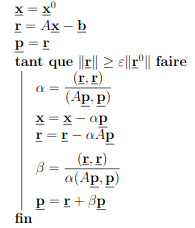
\includegraphics[width=0.6\textwidth]{./Images/Algo1}
		\caption{Algorithme du gradient conjugué muni du test d'arrêt \textbf{t1}}
    \end{minipage}
    \hfill%
    \begin{minipage}[c]{.45\linewidth}
        \centering
        \captionsetup{justification=centering}
        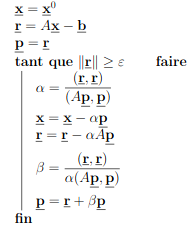
\includegraphics[width=0.6\textwidth]{./Images/Algo2}
		\caption{Algorithme du gradient conjugué muni du test d'arrêt \textbf{t2}}
    \end{minipage}
\end{figure}\vspace{0.3cm}

Le vecteur initial $x_{0}$ a été initialisé au vecteur nul, la tolérance $\varepsilon$ a été fixée à $10^{-10}$ et le vecteur b est choisi tel que la solution du problème $Ax=b$ soit un vecteur contenant uniquement des $1$. En d'autres termes, $b_{i}$ est la résultante des colonnes de la ligne $i$ de la matrice $A$.\\

L'ensemble des matrices testées (à une dimension près) se trouvent en Annexes.

\section{Résultats obtenus}

Convergence des $x_{n}$, convergence des résidus, p.s. des résidus qui forment bien une base, inégalité du conditionnement...

\subsection{Matrices sans perturbation}

Les fichiers de résultats sont obtenus en entrant les données dans un fichier de données puis en donnant en entrée de l’exécutable ce fichier de donnée comme ci-dessous :
\begin{figure}[H]
	\centering
	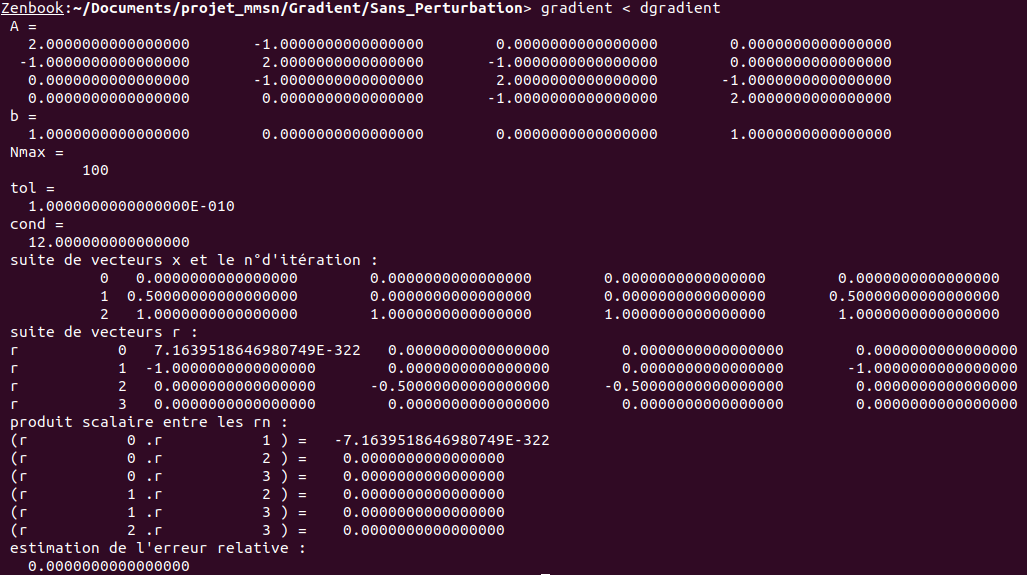
\includegraphics[width=0.75\textwidth]{./Images/dif_4.res}
	\caption{Exemple de fichier de résultat avec une matrice dif\_4 sans perturbation}
\end{figure}

Les propriétés des fichiers de résultat entre les deux tests étant similaires, nous décidons de travailler avec le \textbf{test d'arrêt 1} dans cette partie.


\subsubsection{Matrices dif}

En petites dimensions la suite des $x_{k}$ convergent très rapidement vers la solution, la suite des résidus $r_{k}$ convergent vers 0 assez rapidement et l'estimation de l'erreur relative est très basse. Les résultats en basse dimensions sont peu intéressants.\\

En grandes dimensions, nous observons davantage de résultats. En dimension 50, on observe une convergence de la suite $x_{k}$ plus lente vers la solution. \\

\begin{figure}[htb!]
	\centering
	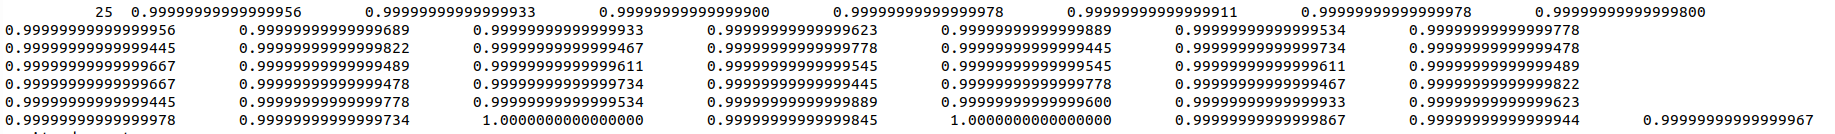
\includegraphics[width=1\textwidth]{./Images/x_dif_50}
	\caption{Vecteur $x_{k}$ à la $25^{eme}$ itération pour $dif_{50}$}
\end{figure}\vspace{0.2cm}

De même pour la suite des résidus $r_{k}$ qui elle converge à la même vitesse que les $x_{k}$. \\

\begin{figure}[htb!]
	\centering
	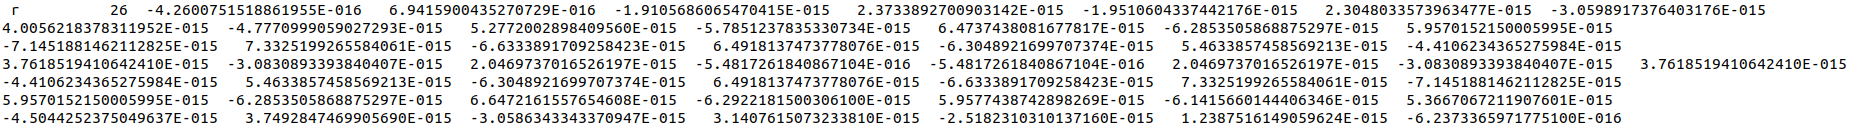
\includegraphics[width=1\textwidth]{./Images/r_dif_50}
	\caption{Vecteur $r_{k}$ à la $26^{eme}$ itération pour $dif_{50}$}
\end{figure}\vspace{0.2cm}

On observe que les composantes du vecteur $r_{k}$ sont très proche de la précision de la machine qui se trouve autour de $10^{-16}$.

Les produits scalaires entre les résidus sont de l'ordre de $10^{-17}$ qui montrent bien l'espace vectoriel engendré par ces derniers qui forment une base orthogonale.

L'erreur relative est de l'ordre de $10^{-15}$ ce qui est très faible, et donc positif pour notre cas.\\

Même en grande dimension, pour cette matrice les convergences sont bien respectées malgré la précision machine.

\subsubsection{Matrice elec}

La matrice étant de petite taille les $x_{k}$ convergent très rapidement vers la solution.\\

\begin{figure}[htb!]
	\centering
	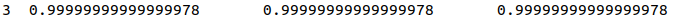
\includegraphics[width=0.8\textwidth]{./Images/x_elec}
	\caption{Vecteur $x_{k}$ à la $3^{eme}$ itération pour $elec$}
\end{figure}\vspace{0.2cm}

De même pour la suite $r_{k}$ qui convergent vers le vecteur nul :

\begin{figure}[htb!]
	\centering
	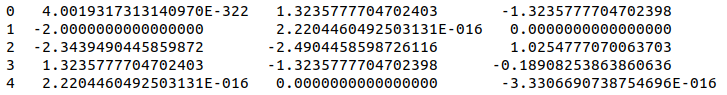
\includegraphics[width=0.8\textwidth]{./Images/r_elec}
	\caption{Vecteurs $r_{k}$ jusqu'à la $4^{eme}$ itération pour $elec$}
\end{figure}\vspace{0.2cm}

En revanche certains produits scalaires sont éloignés de zéro ne formant pas une base orthogonale. 

\begin{figure}[htb!]
	\centering
	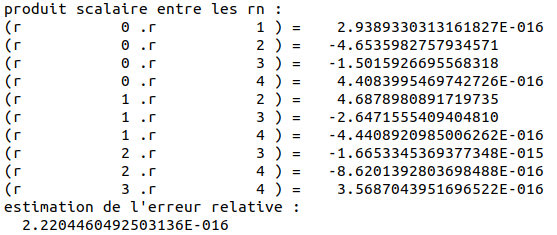
\includegraphics[width=0.8\textwidth]{./Images/ps_elec}
	\caption{Produits scalaires entre les $r_{k}$ pour $elec$}
\end{figure}\vspace{0.2cm}

Cette observation est due aux vecteurs résidus $r_{2}$ et $r_{3}$ qui posent des problèmes d'orthogonalité.\\

On remarque que l'erreur relative est très basse malgré tout.

\subsubsection{Matrice elecmodif}

Cette matrice n'étant pas définie positive il est inutile de l'étudier en profondeur afin de montrer la cohérence avec la partie mathématique attendue numériquement.

Cependant ses propriétés sont étonnantes malgré sa non définie-positivité. En effet ses $x_{k}$ convergent vers la solution, ses vecteurs résidus $r_{k}$ convergent vers le vecteur nul.\\

On retrouve les mêmes produits scalaires anormaux que la matrice elec causés par les vecteurs $r_{2}$ et $r_{3}$ :

\begin{figure}[H]
	\centering
	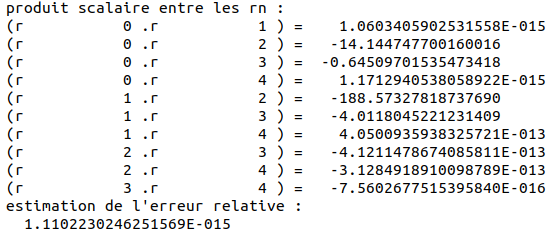
\includegraphics[width=0.8\textwidth]{./Images/ps_elecmodif}
	\caption{Produits scalaires entre les $r_{k}$ pour $elecmodif$}
\end{figure}\vspace{0.2cm}

On remarque que l'erreur relative est également très basse.\\

Même si la matrice n'est pas définie positive, on observe les mêmes propriétés que sa matrice d'origine elec numériquement.

\subsubsection{Matrices de Hilbert}

En dimension 6 la suite des $x_{k}$ et la suite des résidus convergent beaucoup moins rapidement que les matrices précédentes.

\begin{figure}[H]
	\centering
	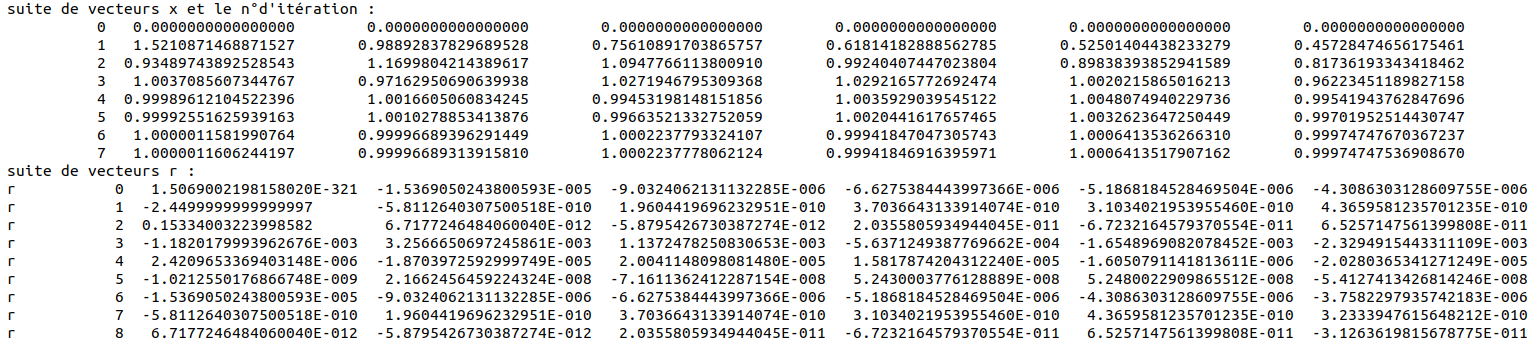
\includegraphics[width=1\textwidth]{./Images/xr_H_6}
	\caption{Convergence des suites $x_{k}$ et $r_{k}$ pour $H_{6}$}
\end{figure}\vspace{0.2cm}

En effet, pour les résidus nous sommes aux alentours de $10^{-12}$ au lieu de $10^{-16}$ dans les exemples précédents. La précision tourne autour de $10^{-5}$ pour le vecteur $x_{k}$ à partir de la $7^{ème}$ itération.\\

Cependant les produits scalaires satisfont bien l'orthogonalité et l'erreur relative est environ $10^{-5}$ ce qui est plutôt élevé par rapport aux exemples précédents.\\

En dimension plus élevée, nous observons les mêmes propriétés. Une convergence des $x_k$ et des $r_k$ assez lente, des produits scalaires au voisinage de zéro et une erreur relative du même ordre.

\subsubsection{Matrice lap}

\begin{figure}[H]
	\centering
	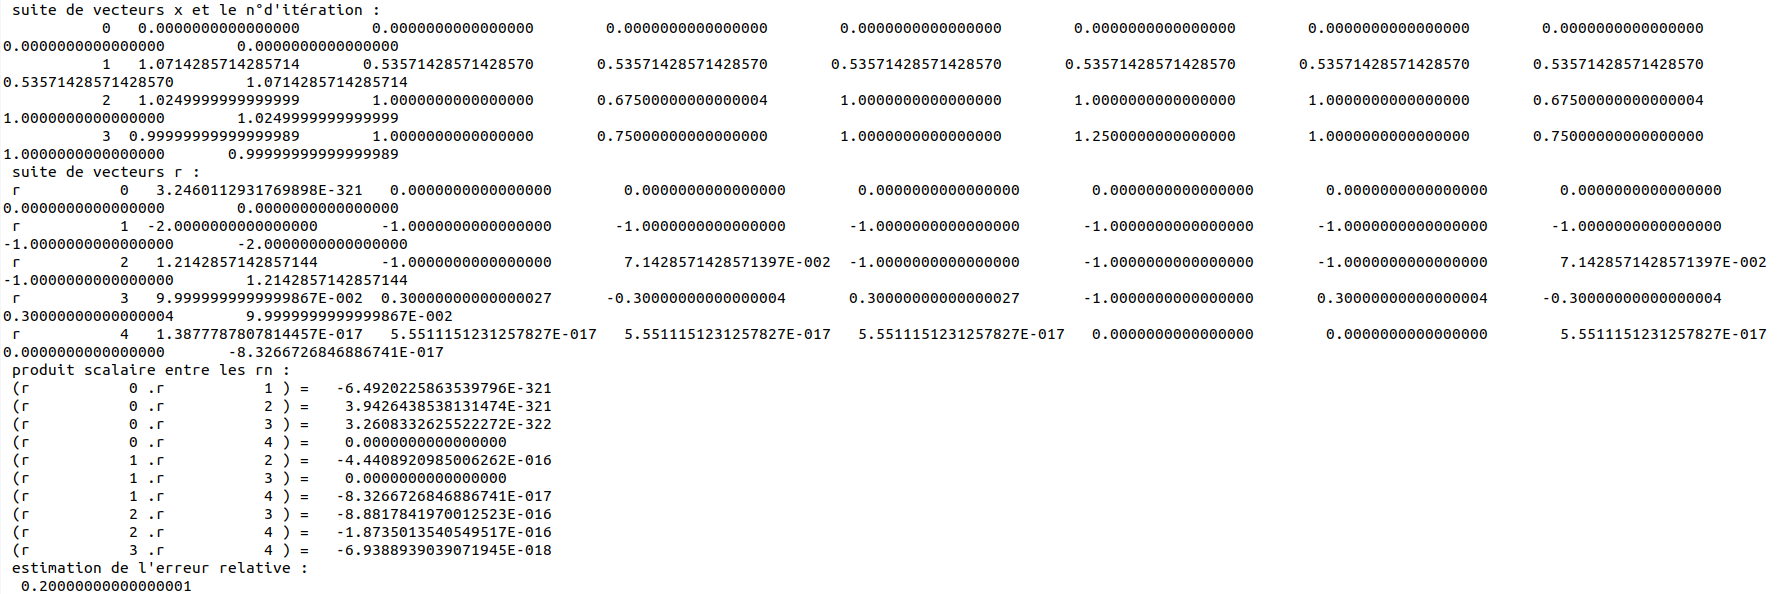
\includegraphics[width=1\textwidth]{./Images/Fichier_res_lap_3}
	\caption{Fichier résultat pour $lap_3$}
\end{figure}\vspace{0.2cm}

La suite des résidus $r_k$ convergent très rapidement vers la limite théorique. Cependant, pour la suite des $x_k$, certaines composantes convergent moins rapidement que d'autres ce qui explique une erreur relative bien au dessus de celles vu précédemment pour les autres matrices.\\

Les produits scalaires sont tous vérifiés et égals à 0 à la précision machine près. L'espace de Krylov engendré par la base orthogonale des résidus $r_k$ pour cette matrice est bien vérifié numériquement

\subsubsection{Matrices $tri_{alpha}$}

Pour ces types de matrice, nous avons décidé de prendre des matrices de dimension 10 avec des $\alpha$ égalent à 2, 5 et 20.\\

Pour les 3 matrices confondues, la convergence est parfaite pour le vecteur solution $x_k$ l'erreur relative. \\

\begin{figure}[H]
	\centering
	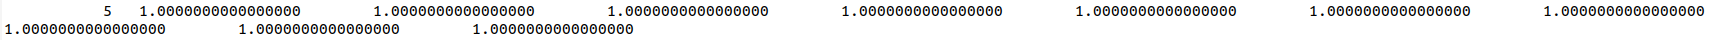
\includegraphics[width=1\textwidth]{./Images/x_tri}
	\caption{Convergence parfaite de la suite $x_k$ à la $5^{ème}$ itération pour les matrices $tri_{alpha_{10}}$}
\end{figure}\vspace{0.2cm}

L'erreur relative est donc nulle pour l'ensemble de ces matrices.\\

Nous observons également une convergence très rapide des résidus et des produits scalaires tous respectés.\\

\begin{figure}[H]
	\centering
	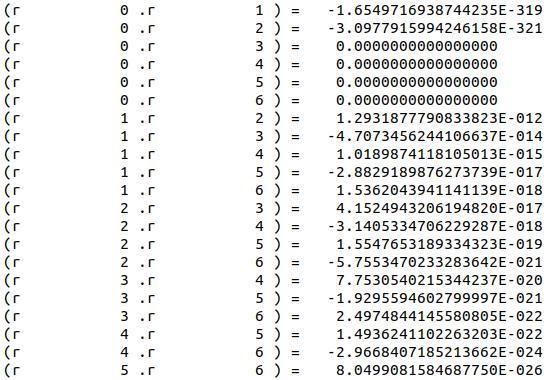
\includegraphics[width=0.5\textwidth]{./Images/ps_tri_20_10}
	\caption{Produits scalaires entre les résidus pour $W$}
\end{figure}\vspace{0.2cm}

La matrice étant très bien conditionnée, le choix du $alpha$ importe peu. Il doit simplement être supérieur à 1 de manière à ce que la matrice soit définie positive.

\subsubsection{Matrice de Wilson}

Pour cette matrice, certains résidus ont du mal à converger vers zéro. En particulier celui à la deuxième itération :\\

\begin{figure}[H]
	\centering
	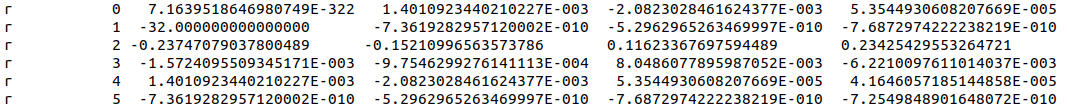
\includegraphics[width=1\textwidth]{./Images/r_W}
	\caption{Suite des résidus $r_k$ pour $W$}
\end{figure}\vspace{0.2cm}

Ce manque de convergence pour certains de ces vecteurs impliquent des produits scalaires très éloignés de 0 et donc des résultats numériques ne permettant pas de vérifier les résultats mathématiques théoriques avec précision.\\

Ce manque de convergence et ce manque de précision sont dus au conditionnement élevé de la matrice carrée de dimension 4.\\

\begin{figure}[H]
	\centering
	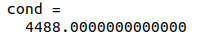
\includegraphics[width=0.2\textwidth]{./Images/Conditionnement_W}
	\caption{Conditionnement de la matrice de Wilson}
\end{figure}\vspace{0.2cm}

Cependant la suite $x_k$ converge assez rapidement vers la solution malgré le conditionnement :\\

\begin{figure}[H]
	\centering
	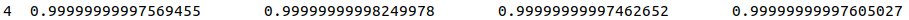
\includegraphics[width=1\textwidth]{./Images/x_W}
	\caption{Vecteur solution $x_k$ à partir de la $4^{ème}$ itération pour $W$}
\end{figure}\vspace{0.2cm}

Enfin l'estimation de l'erreur relative est $10^{-11}$ ce qui est assez faible. 

\subsection{Matrices avec perturbation}

A toi de jouer beau goss \\
De même Les fichiers de résultats sont obtenus en entrant les données dans un fichier de données puis en donnant en entrée de l’exécutable ce fichier de donnée qui contient en plus la matrice de perturbation $\delta$A comme ci-dessous :
\begin{figure}[H]
	\centering
	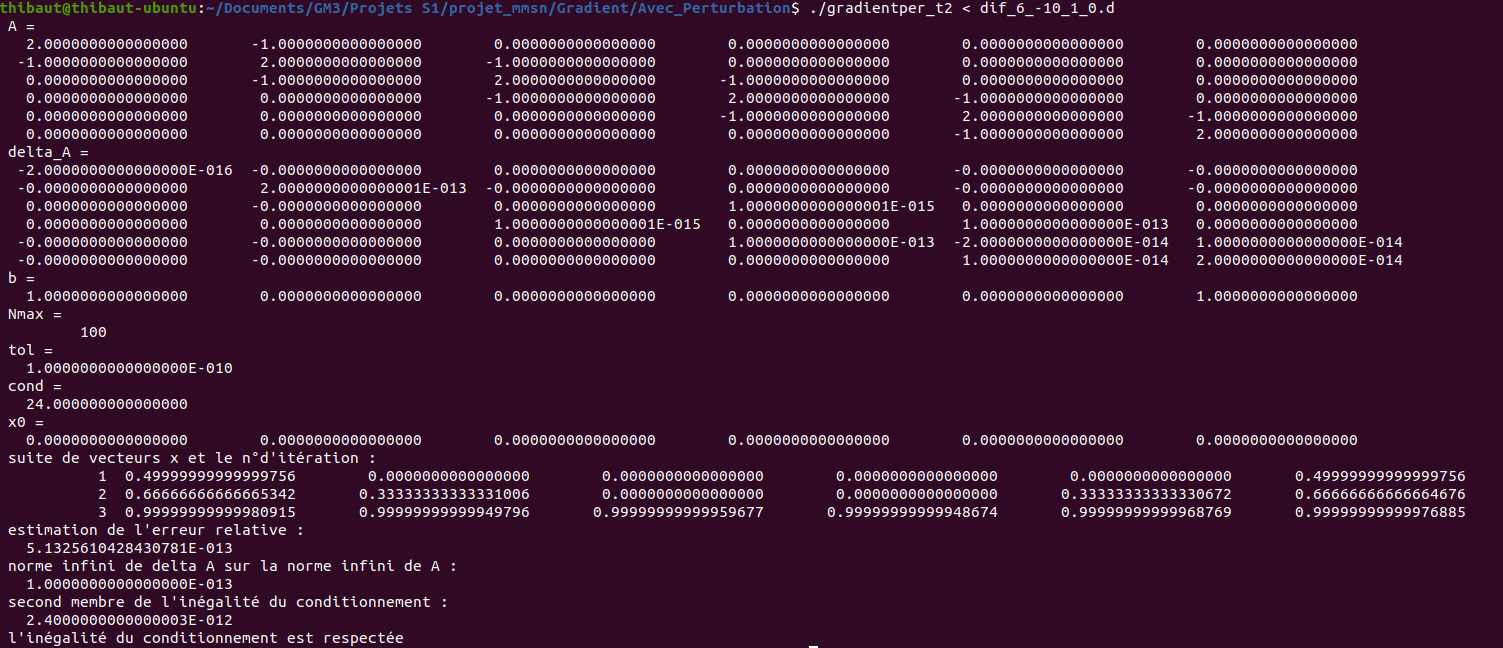
\includegraphics[width=1\textwidth]{./Images/dif_6_1.res}
	\caption{Exemple de fichier de résultat avec une matrice dif\_6 avec perturbation}
\end{figure}

Les propriétés des fichiers de résultat entre les deux tests étant similaires, nous décidons de travailler avec le \textbf{test d'arrêt 2} dans cette partie.

\subsection{Matrices dif}


\chapter*{Conclusion}
\addcontentsline{toc}{chapter}{Conclusion}

Dans la conclusion, vous devez commenter les résultats numériques par rapport á ce que l’on pouvait espérer au vu des résultats théoriques.

Dire qu'avec une complexité comme celle ci (je crois que c'est O(n) ) le gradient conjugué est très apprécié dans des problèmes d'optimisation de grande taille.

\chapter*{Annexes}
\addcontentsline{toc}{chapter}{Annexes}
\addcontentsline{lof}{chapter}{Annexes}
\begin{figure}[H]
    \begin{minipage}[c]{.46\linewidth}
        \centering
        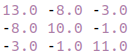
\includegraphics[width=0.5\textwidth]{./Images/elec}\\
        \caption*{Matrice elec}
        \addcontentsline{lof}{section}{Matrice elec}
    \end{minipage}
    \hfill%
    \begin{minipage}[c]{.46\linewidth}
        \centering
        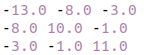
\includegraphics[width=0.5\textwidth]{./Images/elecmodif}\\
        \caption*{Matrice elecmodif}
        \addcontentsline{lof}{section}{Matrice elecmodif}
    \end{minipage}
\end{figure}%\vspace{0.1cm}

\begin{figure}[H]
    \begin{minipage}[c]{.46\linewidth}
        \centering
        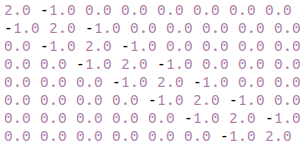
\includegraphics[width=1\textwidth]{./Images/dif_8}\\
        \caption*{Matrice dif de dim 8}
        \addcontentsline{lof}{section}{Matrice dif de dim 8}
    \end{minipage}
    \hfill%
    \begin{minipage}[c]{.46\linewidth}
        \centering
        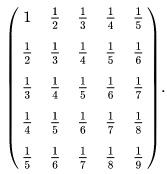
\includegraphics[width=0.6\textwidth]{./Images/H_5}\\
        \caption*{Matrice de Hilbert de dim 5}
        \addcontentsline{lof}{section}{Matrice de Hilbert de dim 5}
    \end{minipage}
\end{figure}%\vspace{0.1cm}

\begin{figure}[H]
    \begin{minipage}[c]{.46\linewidth}
        \centering
        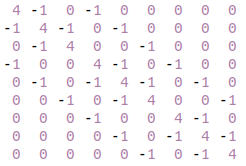
\includegraphics[width=0.9\textwidth]{./Images/lap_3}\\
        \caption*{Matrice Laplacienne\_3 (de dim $3^{2}$)}
        \addcontentsline{lof}{section}{Matrice Laplacienne\_3 (de dim $3^{2}$)}
    \end{minipage}
    \hfill%
    \begin{minipage}[c]{.46\linewidth}
        \centering
        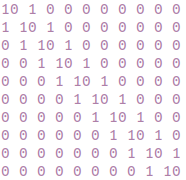
\includegraphics[width=0.6\textwidth]{./Images/tri_5_10}\\
        \caption*{Matrice tri\_$\alpha$ de dim 10 avec $\alpha=5$ }
        \addcontentsline{lof}{section}{Matrice tri\_$\alpha$ de dim 10 avec $\alpha=5$}
    \end{minipage}
\end{figure}%\vspace{0.1cm}

\begin{figure}[H]
	\centering
	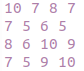
\includegraphics[width=0.17\textwidth]{./Images/W}
	\caption*{Matrice de Wilson}
	\addcontentsline{lof}{section}{Matrice de Wilson}
\end{figure}

\chapter*{Bibliographie}
\addcontentsline{toc}{chapter}{Bibliographie}

	[1] André Draux \textit{Analyse numérique}, poly, chapitre 2 \textit{Les méthodes de descente}.\\

	[2] Maria Kazakova \textit{GM3 Analyse numérique I}, Année 2020-2021, section 1.2.4\\ 
	
	[3] Daniel Kauth \textit{Les méthodes de Krylov} \textit{Optimisation numérique Méthodes du gradient conjugué linéaire}, chapitre 5.1, 5 novembre 2009.

\end{document}
